\documentclass[11pt,a4paper]{article}
\usepackage[utf8]{inputenc}
\usepackage[english]{babel}
\usepackage{graphicx}
\usepackage{fancyhdr}
\usepackage{fullpage}
\setlength{\parindent}{0pt} %no indent after equations or fig. - has to be after TOC
\usepackage{amsmath}
\usepackage{dcolumn}
\usepackage{amsfonts}
\usepackage{amssymb}
\usepackage{graphicx}
\usepackage{wrapfig}
\usepackage{booktabs}
\usepackage[table,xcdraw]{xcolor}
\usepackage{dcolumn}
\usepackage{steinmetz}
\usepackage{float}
\restylefloat{table}
\usepackage{multirow}
\usepackage{listings}
\usepackage{epstopdf}
% hyperlink
\usepackage[linktoc=all]{hyperref}
\hypersetup{
    colorlinks,
    citecolor=black,
    filecolor=black,
    linkcolor=black,
    urlcolor=black
}
\usepackage{wrapfig}
\usepackage{subcaption}
\usepackage{icomma}
\usepackage{setspace}

\usepackage{tocloft}
\renewcommand\cftbeforesecskip{0pt}

\usepackage{color}

\definecolor{dkgreen}{rgb}{0,0.6,0}
\definecolor{gray}{rgb}{0.5,0.5,0.5}
\definecolor{mauve}{rgb}{0.58,0,0.82}

\DeclareCaptionFont{red}{\color{gray}}
\captionsetup{textfont={footnotesize,sc,red},font={footnotesize,sc,red}}

\lstset{frame=false,
  language=C++,
  aboveskip=3mm,
  belowskip=3mm,
  showstringspaces=false,
  columns=flexible,
  basicstyle={\small\ttfamily},
  numbers=left,
  numberstyle=\tiny\color{gray},
  keywordstyle=\color{blue},
  commentstyle=\color{dkgreen},
  stringstyle=\color{mauve},
  breaklines=true,
  breakatwhitespace=true,
  tabsize=3,
  moredelim=**[is][\color{mauve}]{@}{@},
}

\newcolumntype{C}[1]{%
 >{\vbox to 5ex\bgroup\vfill\centering}%
 p{#1}%
 <{\egroup}}  

\graphicspath{{./figures/}}

\title{ROB5}


\begin{document}

\begin{titlepage}
\begin{center}

\textsc{\Large }\\[0.5cm]
\vfill

\includegraphics[scale=0.4]{img/SDU}\\[1cm]
\hrule ~\\[0.3cm]
{ \huge \bfseries The Cup Collector \\ROB5\\[0.4cm] }
\hrule ~\\[1.5cm]
\vfill

% Author and supervisor
\begin{minipage}[t]{7.9cm}
\begin{flushleft} \large
\emph{By:}\\
Jes Jepsen  \\
Keerthikan Ratnarajah\\
Mathias Neerup\\
Nicolai Lynnerup \\
\end{flushleft}
\end{minipage}
\begin{minipage}[t]{7.9cm}
\begin{flushright} \large
\emph{University teacher:} \\
Jimmy Alison Jørgensen \\
jimali@mmmi.sdu.dk
\end{flushright}
\end{minipage}

\vspace{1.2cm}
Dato: \today


\end{center}
\end{titlepage}

\tableofcontents
\newpage

\newpage
\section{The Cup Collector}
The cantina at SDU has in a period of time collected empirical data that suggests that researchers and students at SDU are lazy and forgetful when it comes to bringing back used cups to the cantina. To avoid situations where there are no coffee cups and thereby loosing coffee sales (or fresh students), the cantina has decided to assign the task of collecting cups form offices and hallways of SDU, to one person for 2 hours per day.\\[0.2cm]
A master student with some knowledge on vision and point clouds has using a Kinect and a robot arm implemented an algorithm to detect and collect cups within a distance of 2 meters. Also he has implemented the stable grasping of cups that are within 1 meter of the robot. Unfortunately, this master student never attended ROB05 and therefore has no skill in navigating robots.\\[0.2cm]
The problem is therefore presented to this year’s class in ROB05.\\[0.2cm]
The task contains 3 parts. All 3 must be targeted in the project.

\subsection{Limitations and information}
\begin{itemize}
\item The map ”complete\_map\_project.pgm” use a scale 10pixel:1m and figure \ref{fig::original} shows the complete map. 
\item The map use the scale 10px to 1 meter
\item The robot can only carry 20 cups at the time
\item The robot is NOT a point robot. It has a circular shape with a radius of 0.4m, which in this map then is equivalent to a radius of 4px. 
\item The robot can drive up to 5km per hour
\item The elevators are denoted with pixelvalues 128,129,130,131 and 132.
\end{itemize}

\begin{figure}[H]
\centering
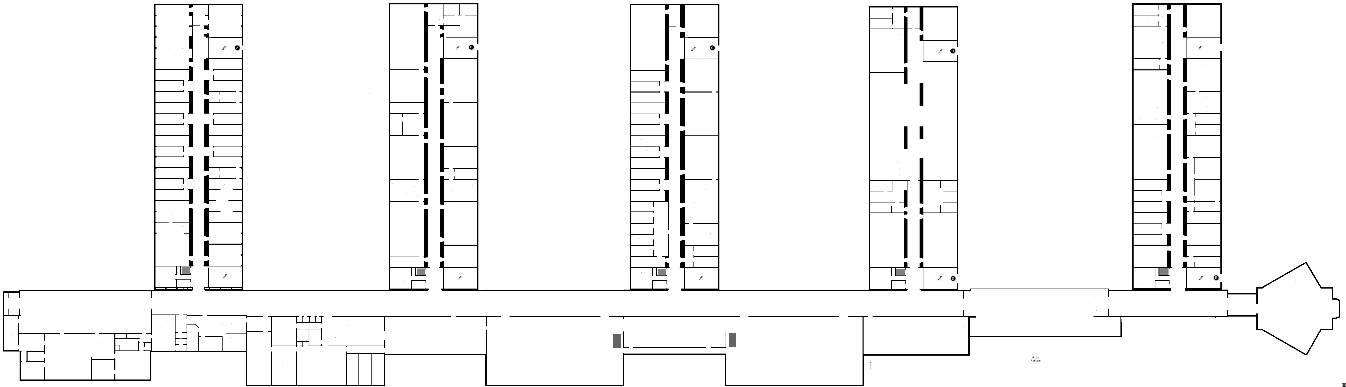
\includegraphics[scale=0.33]{img/original.png}
\caption{The complete map of SDU.}
\label{fig::original}
\end{figure}

\newpage

\section{Planning}
\label{sec::planning}
All rooms in the map must be checked in order to find cups. The robot must be within 2 meters of a cup in order to actually detect the cup and within 1 meter in order to collect it. Cups are marked in the map using one pixel with grayscale value 150. Cups can be unloaded at the two offloading stations in the cafeteria. The offloading stations are represented with pixel values 100. The robot must start and end at an offloading station.\\[0.2cm]
You are free in regard in choice of algorithms. However, please document what algorithm you choose, how many kilometers the robot moves and how long it takes to calculate the path the robot takes.\\[0.2cm]
All planning is done offline, and it involves the functions:
\begin{itemize}\itemsep-2pt
\item \textbf{Wavefront} from the two unloading--stations
\item \textbf{Detection} of the rooms and blocks
\item \textbf{Priority queues} for each block and the
\end{itemize}

\subsection{Solution}
The first thing that happens in the planning part, is that a wavefront is generated from the two positions where the unloading--stations are located in the cafeteria. Cups are also seen as obstacles, when the wavefront is generated. The pixel values for the two unloadings stations are 
\begin{eqnarray*}
Unloading-station\: 1&:& \hspace{1cm}(3100,1400) \\
Unloading-station\: 2&:& \hspace{1cm}(2150,1400) \\
\end{eqnarray*}
and figure \ref{fig::path} shows how the wavefront expands from the two unloading--stations in the complete map. The unloading stations are the two darkest areas on the figure.\\[.2cm]
The wavefront--values is stored in a 2D--array, so when it is time for emptying the container, it is possible run the wavefront--function quickly in the online part. The generated array takes up some memory, but it saves time keeping the wavefront--map to the two unloading stations. When the cup container is filled, a path to the nearest unloading--station is found by using the offline wavefront function, \lstinline|makeWaveFrontoffline(currentX,currentY)|. For each pixel the robot moves through the wavefront path to a station, each coordinate is pushed into a vector--pair, so it can take the same path back to where it were interrupted by popping the values from the vector--pair. Just like Hansel and Gretel with the breadcrumbs, except that the robot will not get lost in the woods, find a gingerbread house, be fattened and so on.  

\begin{figure}[H]
\centering
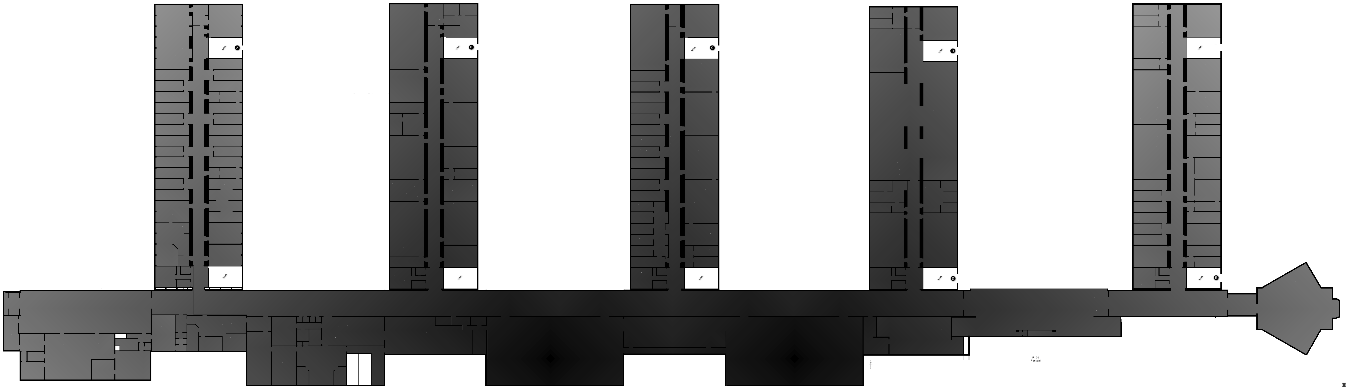
\includegraphics[scale=0.33]{img/wavefront_path.png}
\caption{How the wavefront expands from the two unloading--stations in the complete map.}
\label{fig::path}
\end{figure}

Detection of a room has four steps
\begin{enumerate}\itemsep-3pt
\item First the upper left corners ($C_{ul}$) of the squares are detected. Each pixel in the map is checked with a 3x3--mask, shown in table \ref{tab::ul_mask}, which looks at if the pixel value neighbors are obstacles, which corresponds to a left corner. If the mask matches, then the pixel is marked as a $C_{ul}$ and the position for the pixel is stored in a data type, called \lstinline|square|. 

\begin{table}[H]
\centering
\begin{tabular}{|l|l|l|}
\hline
0 & 0 & 0 \\ \hline
0 & P &   \\ \hline
0 &   &   \\ \hline
\end{tabular}
\caption{3x3 mask for detecting upper left corners}
\label{tab::ul_mask}
\end{table}

\item Next the upper right corners ($C_{ur}$) is found by taking the the position for each $C_{ul}$, and then keep moving to the right, until it hits an obstacle. When it hits an obstacle, the pixel just before is marked as a $C_{ur}$ and stored in \lstinline|square|. On table \ref{tab::corner_detection} is this approach shown.
\item Next the lower left corners $C_{ll}$ is found, just like the $C_{ur}$, by taking the the position for each $C_{ul}$, but instead it keeps moving down, until it hits an obstacle. When it hits an obstacle, the pixel just before is marked as a $C_{ll}$ and stored in \lstinline|square|. On table \ref{tab::corner_detection} is this approach shown. 
\item The lower right corner ($C_{lr}$) is not detected like the other three corners, it is calculated by taking the height distance (in pixels) between $C_{ul}$ and $C_{ll}$, and assuming that the $C_{lr}$ has the same height distance from the $C_{ur}$. Like the other corners, the $C_{lr}$ is marked and stored in \lstinline|square|. 
\end{enumerate} 

\begin{table}[H]
\centering
\begin{tabular}{|c|
>{\columncolor[HTML]{C0C0C0}}c ccccccc|c|}
\hline
\cellcolor[HTML]{000000}{\color[HTML]{FFFFFF} 0} & \multicolumn{1}{l|}{\cellcolor[HTML]{000000}{\color[HTML]{FFFFFF} 0}} & \multicolumn{1}{l|}{\cellcolor[HTML]{000000}{\color[HTML]{FFFFFF} 0}} & \multicolumn{1}{l|}{}            & \multicolumn{1}{l|}{}            & \multicolumn{1}{l|}{}            & \multicolumn{1}{l|}{}            & \multicolumn{1}{l|}{}            &                                  &                                                  \\ \hline
\cellcolor[HTML]{000000}{\color[HTML]{FFFFFF} 0} & \cellcolor[HTML]{9B9B9B}$C_{ul}$                                      & \cellcolor[HTML]{C0C0C0}$\cdots$                                      & \cellcolor[HTML]{C0C0C0}$\cdots$ & \cellcolor[HTML]{C0C0C0}$\cdots$ & \cellcolor[HTML]{C0C0C0}$\cdots$ & \cellcolor[HTML]{C0C0C0}$\cdots$ & \cellcolor[HTML]{C0C0C0}$\cdots$ & \cellcolor[HTML]{9B9B9B}$C_{ur}$ & \cellcolor[HTML]{000000}{\color[HTML]{FFFFFF} 0} \\ \cline{1-1} \cline{10-10} 
\cellcolor[HTML]{000000}{\color[HTML]{FFFFFF} 0} & $\vdots$                                                              & \cellcolor[HTML]{C0C0C0}                                              & \cellcolor[HTML]{C0C0C0}         & \cellcolor[HTML]{C0C0C0}         & \cellcolor[HTML]{C0C0C0}         & \cellcolor[HTML]{C0C0C0}         & \cellcolor[HTML]{C0C0C0}         & \cellcolor[HTML]{C0C0C0}$\vdots$ &                                                  \\ \cline{1-1} \cline{10-10} 
                                                 & $\vdots$                                                              & \cellcolor[HTML]{C0C0C0}                                              & \cellcolor[HTML]{C0C0C0}         & \cellcolor[HTML]{C0C0C0}         & \cellcolor[HTML]{C0C0C0}         & \cellcolor[HTML]{C0C0C0}         & \cellcolor[HTML]{C0C0C0}         & \cellcolor[HTML]{C0C0C0}$\vdots$ &                                                  \\ \cline{1-1} \cline{10-10} 
                                                 & \cellcolor[HTML]{9B9B9B}$C_{ll}$                                      & \cellcolor[HTML]{C0C0C0}$\cdots$                                      & \cellcolor[HTML]{C0C0C0}$\cdots$ & \cellcolor[HTML]{C0C0C0}$\cdots$ & \cellcolor[HTML]{C0C0C0}$\cdots$ & \cellcolor[HTML]{C0C0C0}$\cdots$ & \cellcolor[HTML]{C0C0C0}$\cdots$ & \cellcolor[HTML]{9B9B9B}$C_{lr}$ &                                                  \\ \hline
                                                 & \multicolumn{1}{l|}{\cellcolor[HTML]{000000}{\color[HTML]{FFFFFF} 0}} & \multicolumn{1}{l|}{}                                                 & \multicolumn{1}{l|}{}            & \multicolumn{1}{l|}{}            & \multicolumn{1}{l|}{}            & \multicolumn{1}{l|}{}            & \multicolumn{1}{l|}{}            &                                  &                                                  \\ \hline
\end{tabular}
\caption{Detection of the room corners}
\label{tab::corner_detection}
\end{table}

When all the rooms are detected, the center of each room is calculated, by taking the half of the weight and height of the room, and stores it as a vector--pair. Each room in the list is then check wherever a room is actually a room or a hallway by looking at the relationship between the wall of the room. Some thresholds are set, so if the relationship excites these threshold, then the room is detected as a hallway instead. On figure \ref{fig::graph} can it be seen how the different rooms are connected to each hallway. The hallways has a priority queue, which prioritizes the room after the distance between the center of the hallway to the center of the room. Each room is put in the priority queue of that hallway center that is closest to the center of the room. This priority for each hallway is the order of which room that are cleaned and emptied for cups first.

\begin{figure}[H]
\centering
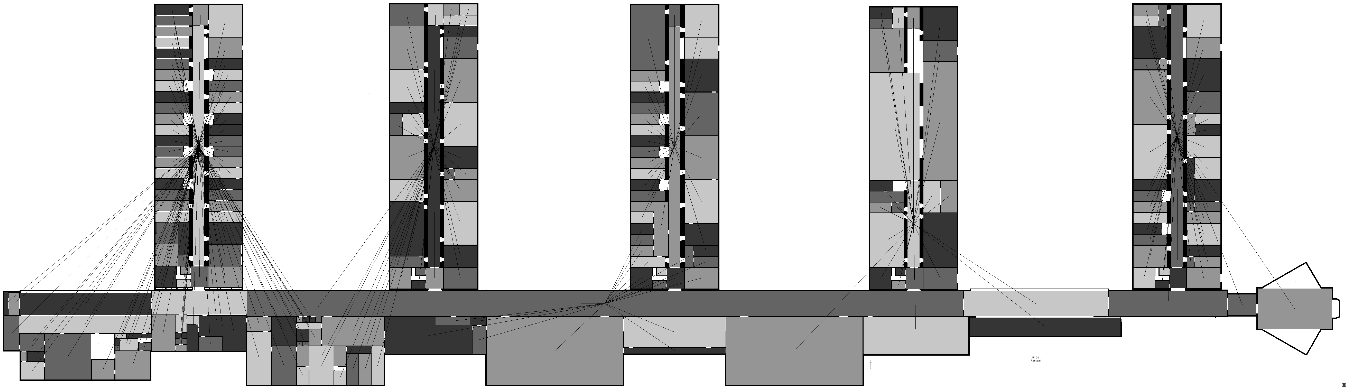
\includegraphics[scale=0.33]{img/graph.png}
\caption{An overview of how the different rooms are detected and connected to each hallway on the complete map of SDU.}
\label{fig::graph}
\end{figure}

\subsection{Results}

\subsection{Alternatives}
As alternatives to planning could be the following methods may also be used:
\begin{itemize}\itemsep-2pt
\item Sweepline
\end{itemize}

\newpage

\section{Coverage}
\label{sec::coverage}
The Dean feels that it is not economically justified to by a robot system for 80.000 euro just to collect cups. Hence, it is interesting to have the robot do a second task, namely washing of the floors. Therefore calculate a coverage path that covers most of the floor in the map. Again the robot must start and end at the offloading stations.\\[0.2cm]
Again, you are free to choose algorithm and you should document the choice, the distance in kilometres that the robot moves and how long it takes to compute the coverage path.

All coverage is done online, and it involves the functions
\begin{itemize}\itemsep-2pt
\item \textbf{Wavefront} from the robots current position to the center of an other room
\end{itemize}

\subsection{Method}
The coverage plan for the complete map is
\begin{enumerate}\itemsep-2pt
\item Block A
\item The Big Hall
\item Block B
\item Block C
\item Block D
\item Block E
\end{enumerate}

Figure \ref{fig::room} illustrates covering a room. The dark gray pixels are where the robot is moving and the light gray area is what the robot has covered. The coverage is done in the following steps
\begin{enumerate}\itemsep-2pt
\item Starts at upper left corner of the rooms freespace, $Q_{room}$, and keep moving down to the lower left corner of the $Q_{room}$.
\item Turn left 90 degrees and move 8 pixels
\item Turn left 90 degrees and keep moving until the limit of the $Q_{room}$ is detected.
\item Turn right 90 degrees and move 8 pixels
\item Turn right 90 degrees and keep moving until the limit of the $Q_{room}$ is detected.
\item Keep repeating the step 2 to 5 until the same y--coordinate as the upper right corner of the rooms $Q_{room}$ is detected. At this point, either the robot has the same position as the upper right corner or the lower right corner of the $Q_{room}$.    
\begin{itemize}\itemsep-2pt  
\item If it is position of the lower right corner of the $Q_{room}$, then turn 90 degrees to the left and keep moving until the robot has the same position as the upper right corner of the $Q_{room}$ (Case A on figure \ref{fig::room}). The room is fully covered and the robot can move to the next room. 
\item If it is position of the upper right corner of the $Q_{room}$, then turn right 90 degrees and keep moving until the robot has the same position as the lower right corner of the $Q_{room}$ (Case B on figure \ref{fig::room}). The room is fully covered and the robot can move to the next room. 
\end{itemize}
\end{enumerate} 
When the room is fully covered, then the center of the next room is popped from the priority queue of the block, that the robot is currently in. A wavefront is then generated from that center-position, until the wavefront hits the position of the robot, and then the path to that center is found. The wavefront is stopped as soon as it hits the robots position, because the robot will never gonna use the rest of wavefront, and it saves a lot of time and memory by not making a full wavefront map. This makes it also possible to run the wavefront online, because most often the robot does not have to drive so far to get to the next room center. 

\begin{figure}[H]
\centering
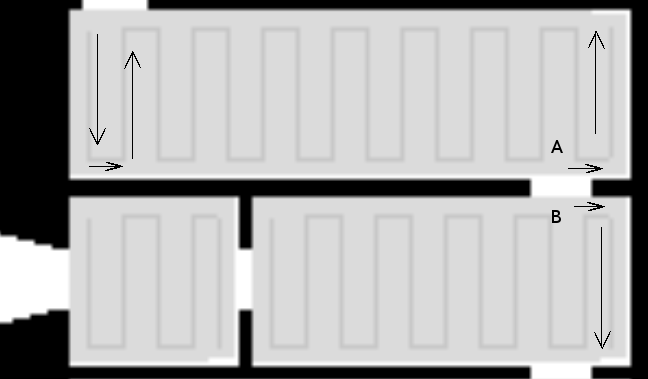
\includegraphics[scale=0.33]{img/room.png}
\caption{Coverage of a room in the complete map.}
\label{fig::room}
\end{figure}

Figure \ref{fig::coverage} shows the complete map fully covered.

\begin{figure}[H]
\centering
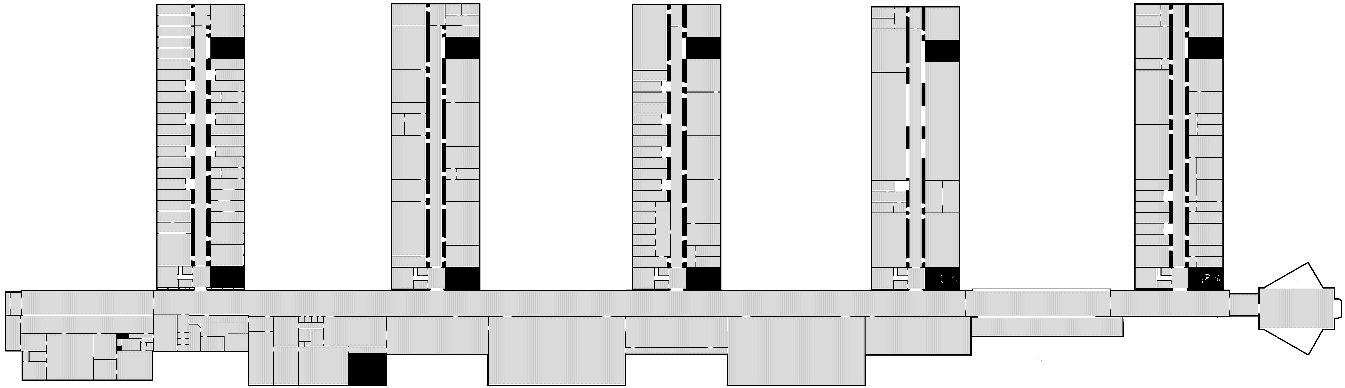
\includegraphics[scale=0.33]{img/coverage.png}
\caption{Coverage of a room in the complete map.}
\label{fig::coverage}
\end{figure}

\subsection{Results}

\subsection{Conclusion}
What works and what does not? Why?

\newpage

\section{Localization}
\label{sec::localisation}
Finally, a method to compute the state (configuration) of the robot is required. The method should be applied to a real system such as the Nexus platform from the course and due to the size of the university it is important that the robot is able to use features to precisely measure its whereabouts. These features could be based on the Hokoyo 2D laser scanner mounted on the robot.\\[0.2cm]
Again document what algorithm, and test how well it performs. You should at least write what model you choose for the robot and show that the localisation works better than odometry alone.\\[0.2cm]
In the real world, no actuator is perfect: they may overshoot or undershoot the desired amount of motion. So when a robot tries to drive in a straight line, it will inevitably curve to one side or the other due to minute differences in wheel radius. Figure \ref{fig::MC_test} shows how the position of a robot can get more and more uncertain, as it moves in straight lines. A robot becomes less sure of its position if it moves blindly without sensing the environment, so it is necessary to sensors to localize the robot in the environment, and not only count on the odometry alone. To solve this, on the robot is a 2D laser range scanner mounted to sense the environment around it.
\begin{figure}[H]
\centering
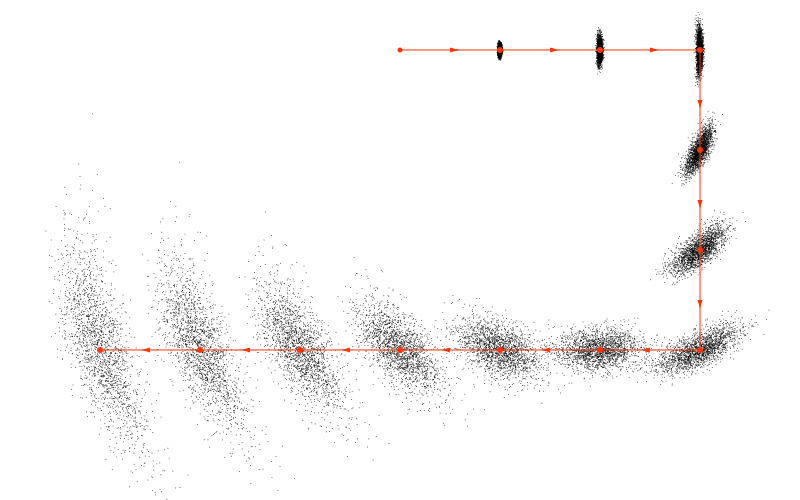
\includegraphics[scale=0.43]{img/MCtest.png}
\caption{Belief after moving several steps for a 2D robot using a typical motion model without sensing.}
\label{fig::MC_test}
\end{figure}
All localization is done online, and it involves the functions:
\begin{itemize}\itemsep-2pt
\item \textbf{Monte Carlo localization (MCL)} for determining the localization of the robot as it moves. This algorithm is normally used for robots to localize using a particle filter.
\item \textbf{Set linear speed} for the robot, to determine how fast it should move
\item \textbf{Set rotations speed} on each wheel of the robot, so it possible for it to turn 90 degrees to either left or right.  
\end{itemize}
\newpage
\subsection{Solution}
The MCL is given a map of the environment, and then the algorithm estimates the position and orientation of a robot as it moves and senses the environment. This is used to determine the position of the robot, by following\footnote{\url{http://en.wikipedia.org/wiki/Monte_Carlo_localization}} 
\begin{enumerate}\itemsep-2pt
\item The algorithm uses a particle filter to represent the distribution of likely states, with each particle representing a possible state, i.e. a hypothesis of where the robot is. First $N$ numbers of normal distributed hypothesis of the robots position is made of the entire map. At this point, the robot has no information about where it is and can only assumes it is equally likely to be at any point in configuration space.
\item All the hypothesis is compared to what the 2D laser range scanner sees, and that hypothesis with the highest probability, i.e. how well the actual sensed data correlate with the predicted position, an is assumed being the robots current position.
\item Whenever the robot moves, it shifts the particles to predict its new state after the movement, so, $N$ normal distributed hypotheses surrounding our current position--hypothesis is made within a smaller area around the predicted current position. Maintaining the entire map as sample size would be computationally wasteful and make the the calculations less precise.
\item Step 2 to 4 is repeated with the previous belief as input, because ultimately, the particles should converge towards the actual position of the robot. This is repeated until the robot is either turned off or done collecting the cups.
\end{enumerate}
Figure \ref{fig::MC} shows the implemented Monte Carlo method on the robot. The yellow dots are the hypothesis that is normal distributed around the robot and the red dot is the robots current position according to the hypothesis and what the 2D laser range scanner sees. All white pixels are free space and the black pixels are obstacles. The robot is seen as a point--robot in this example.\\[0.2cm]

\begin{figure}[H]
\centering
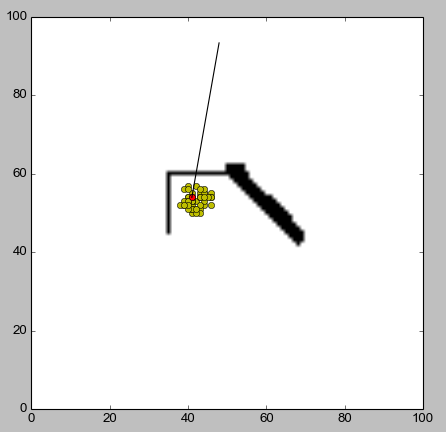
\includegraphics[scale=0.43]{img/MC.png}
\caption{Monte Carlo hypothesis (yellow dots) and the current position (red dot)}
\label{fig::MC}
\end{figure}

\newpage
\subsection{Results}
How long does it take?

\subsection{Alternatives}
As alternatives to localization could the following methods may also be used:
\begin{itemize}\itemsep-2pt
\item Kalman filter
\end{itemize}


\newpage

\section{Future work}
Use a greedy algorithm. 

















































\end{document}